% to choose your degree
% please un-comment just one of the following
\documentclass[bsc,frontabs,twoside,singlespacing,parskip,deptreport]{infthesis}     % for BSc, BEng etc.
% \documentclass[minf,frontabs,twoside,singlespacing,parskip,deptreport]{infthesis}  % for MInf
\usepackage{hyperref}
\usepackage{graphicx}
\usepackage{booktabs, multirow} % for borders and merged ranges
\usepackage{soul}% for underlines
\usepackage[table]{xcolor} % for cell colors
\usepackage{changepage,threeparttable} % for wide tables
\usepackage{pgfplots}

\graphicspath{ {./figures/} }

\begin{document}

\title{Multicore Processing Support \\ for a Research Operating System}

\author{Kimberley Stonehouse}

% to choose your course
% please un-comment just one of the following
% \course{Artificial Intelligence and Computer Science}
%\course{Artificial Intelligence and Software Engineering}
%\course{Artificial Intelligence and Mathematics}
%\course{Artificial Intelligence and Psychology }   
%\course{Artificial Intelligence with Psychology }   
%\course{Linguistics and Artificial Intelligence}    
\course{Computer Science}
%\course{Software Engineering}
%\course{Computer Science and Electronics}    
%\course{Electronics and Software Engineering}    
%\course{Computer Science and Management Science}    
%\course{Computer Science and Mathematics}
%\course{Computer Science and Physics}  
%\course{Computer Science and Statistics}    

% to choose your report type
% please un-comment just one of the following
%\project{Undergraduate Dissertation} % CS&E, E&SE, AI&L
%\project{Undergraduate Thesis} % AI%Psy
\project{4th Year Project Report}

\date{\today}

\abstract{
This is an example of {\tt infthesis} style.
The file {\tt skeleton.tex} generates this document and can be 
used to get a ``skeleton'' for your thesis.
The abstract should summarise your report and fit in the space on the 
first page.
%
You may, of course, use any other software to write your report,
as long as you follow the same style. That means: producing a title
page as given here, and including a table of contents and bibliography.
}

\maketitle

\section*{Acknowledgements}
Acknowledgements go here. 

\tableofcontents

%\pagenumbering{arabic}


\chapter{Introduction}

The document structure should include:
\begin{itemize}
\item
The title page  in the format used above.
\item
An optional acknowledgements page.
\item
The table of contents.
\item
The report text divided into chapters as appropriate.
\item
The bibliography.
\end{itemize}

Commands for generating the title page appear in the skeleton file and
are self explanatory.
The file also includes commands to choose your report type (project
report, thesis or dissertation) and degree.
These will be placed in the appropriate place in the title page. 

The default behaviour of the documentclass is to produce documents typeset in
12 point.  Regardless of the formatting system you use, 
it is recommended that you submit your thesis printed (or copied) 
double sided.

The report should be printed single-spaced.
It should be 30 to 60 pages long, and preferably no shorter than 20 pages.
Appendices are in addition to this and you should place detail
here which may be too much or not strictly necessary when reading the relevant section.

\section{Using Sections}

Divide your chapters into sub-parts as appropriate.

\section{Citations}

Note that citations 
(like \cite{P1} or \cite{P2})
can be generated using {\tt BibTeX} or by using the
{\tt thebibliography} environment. This makes sure that the
table of contents includes an entry for the bibliography.
Of course you may use any other method as well.

\section{Options}

There are various documentclass options, see the documentation.  Here we are
using an option ({\tt bsc} or {\tt minf}) to choose the degree type, plus:
\begin{itemize}
\item {\tt frontabs} (recommended) to put the abstract on the front page;
\item {\tt twoside} (recommended) to format for two-sided printing, with
  each chapter starting on a right-hand page;
\item {\tt singlespacing} (required) for single-spaced formating; and
\item {\tt parskip} (a matter of taste) which alters the paragraph formatting so that
paragraphs are separated by a vertical space, and there is no
indentation at the start of each paragraph.
\end{itemize}

\chapter{Background}

% \section{Motivation} \label{motivation}
\section{Unicore Limitations} \label{unicore-limitations}
% What led to the development of multicore processing?
Moore’s Law predicts that the number of transistors per integrated circuit doubles roughly every two years \cite{moore_1998} \cite{moore_2006}. For decades, Moore’s Law scaling has correctly predicted exponential advancements in computing performance, which has set a precedent. However, this doubling cannot go on forever, and Moore’s law is coming to an end \cite{DBLP:journals/cse/TheisW17}. Still, our expectations have been set, and so the computing industry has begun to look to new ways of improving computing performance. This has ultimately introduced two key issues.

\subsection{The Power Wall} \label{the-power-wall}
In a processor, the operations performed are governed by a system clock, with each operation beginning on a pulse of the clock. These operations may include fetching an instruction, decoding an instruction or performing an arithmetic operation. It follows that fundamentally, the speed of the processor is determined by the speed of the clock, so chip manufacturers have historically improved performance by increasing the clock speed \cite{stallings}.

In part, increasing the clock speed was made possible by Dennard scaling \cite{dennard_1999}, which suggests that as transistors get smaller, their power density stays constant, so that power use stays in proportion with the chip's area. This should have allowed circuits to operate at higher frequencies without increasing the power usage. However, this scaling rule ignored transistor leakage, which aggregates with a growing number of increasingly small transistors and drives up power consumption \cite{bohr_2007}.

This breakdown of Dennard scaling meant that increasing performance in this manner demands an increase in power, which is problematic. As an example, the digital workload of mobile phones increases by an order of magnitude by every 5 years, demanding performance improvement. However, the dominant constraining factor is the limited available battery power \cite{berkel_2009}. In larger applications such as servers and data centres, the dominant constraining factor becomes running costs, which are driven up by excessive power consumption. The breakdown of Dennard scaling has effectively defined a “power wall” \cite{patterson-hennessy}. Power consumption has become a limiting factor, and the trend described above of ever-increasing clock speeds is unsustainable \cite{blake_2009}.

\subsection{Performance Growth} \label{performance-growth}
Performance can also be improved by increasing the logic complexity on the chip. For example, superscalar processors are used to implement instruction-level parallelism to improve performance. That is, they contain multiple instances of execution units such as the ALU. Each execution unit is not a separate processor, but simply an additional resource of the existing processor. This allows for multiple instructions to be executed in parallel within the same processor, increasing throughput \cite{stallings}.

However, there are diminishing returns here: Pollack’s rule states that the performance increase delivered by microarchitectural improvements is roughly proportional to the square root of the increase in logic complexity \cite{borkar_2007}. In other words, doubling the logic in the processor will result in roughly a 40\% increase in performance. To illustrate this fact, we can look at the trend of yearly chip performance improvement. In the 1990s, chip performance was improving by 60\% each year, but this slowed to 40\% each year between 2000 to 2004, and slowed again to 20\% in 2004 \cite{geer_2005}. Clearly, increasing the complexity of processor designs is a poor investment.

\section{Towards Multicore} \label{towards-multicore}
% What is multicore processing?
A mulitcore architecture can address the two key issues discussed above. A multicore processor has two or more processing units, called cores, on the same chip. Different to superscalar processors, each core has all the components of an independent processor, including registers, control unit, arithmetic logic unit, instruction pipeline and private L1 cache. The cores also have access to a shared L2 cache, and increasingly, a shared L3 cache. Each core appears to the operating system as a separate processor. 

Performance growth can then come from increasing the number of cores rather than the clock speed. Using multiple cores rather than one increasingly powerful core has a slower growth in power consumption \cite{blake_2009}, meaning that in the case of mobile phones, which are constrained by battery power, the solution has to be multicore \cite{berkel_2009}. A multicore architecture also has the potential to provide a nearly linear performance improvement with complexity. For example, two smaller processor cores instead of one monolithic core can provide a 70-80\% performance improvement, compared to the 40\% mentioned previously \cite{borkar_2007}.

Chip manufacturers soon turned to multicore. In 2001, IBM released the POWER4, the industry’s first server chip with two cores \cite{power4}. In 2005, AMD announced the first dual-core Opteron, their server processor. A month later came the Athlon 64 X2, AMD’s first desktop dual-core processor. Today, the multicore trend shows no signs of slowing down. The Fujitsu A64FX has 48 cores and powers the Fugaku supercomputer \cite{a64fx}, which was the fastest supercomputer in the world as of June 2020 \cite{top500}. The Sunway TaihuLight supercomputer has 256 cores per processor chip, amounting to over 10 million cores across the entire system \cite{sunway}. However, despite being prevalent, multicore processing presents a number of challenges, discussed along with relevant technical concepts below.

\subsection{Architecture} \label{architectural-challenges}
An instruction set architecture (ISA) is an abstract model of a computer that defines the type of instructions to be supported by the processor. Examples include x86, ARM, RISC-V and MIPS. A microarchitecture is the design of a particular processor, which implements a specific ISA. Processors may have different microarchitectures, but share a common ISA. For example, the AMD Athlon and the Intel Core processors have entirely different designs, but both implement the x86 ISA with only minor differences.

The ISA will sometimes present a multiple processor (MP) protocol, which defines how the cores interact with one another. However, this is not always the case, and notably the MIPS and RISC-V ISAs do not have mature MP protocols. This shifts the decision about core interaction onto the operating system designer, adding complexity to the design and development of the operating system. The ARM ISA does not have a standardised MP protocol, and so the implementation is left to the developer. Microsoft did propose a protocol in 2014, but this has not been widely adopted. Instead, most developers use the Generic Interrupt Controller (GIC) to interact with the cores.

The x86 ISA does define a multiple-processor (MP) initialisation protocol called the Multiprocessor Specification Version 1.4 \cite{intel-sys-prog-guide}. The protocol defines two classes of processors: the bootstrap processor (BSP) and application processors (APs). If one core requires action from another core, it can send a special type of interrupt, called an inter-processor interrupt (IPI). When the MP system is powered on, the system hardware dynamically selects one of the processors as the BSP, and the remaining processors are identified as APs. The BSP executes the BIOS’s bootstrap code and then the operating-system initialisation code, while the APs wait for a sequence of IPIs from the BSP processor. The sequence, called an INIT-SIPI-SIPI sequence, consists of one init IPI followed by two startup IPIs, with delays throughout to allow the APs time to respond.

Even with a multiple processor standard, there still remains the issue of how to organise multiple cores. A homogeneous architecture consists of a number of processing cores of the same microarchitecture and ISA. Conversely, a heterogeneous architecture consists of processing cores of different microarchitectures, capabilities and perhaps ISAs, with each core being suited to a certain set of tasks.

Heterogeneous architectures can offer improved performance. To fully exploit the benefits of multicore processing, software must be highly adapted to a parallel execution environment (discussed further in section \ref{scalability-challenges}). The programmer's effort to parallelise the program can be reduced if the underlying architecture promises faster execution of the serial part of an application \cite{suleman_2007}. Consider, for example, a system with many simple cores to provide high parallelisation, and a few complex cores to ensure high serial performance too \cite{balakrishnan_2005}. 

Core diversity can also offer a greater ability to adapt to the demands of different applications, and running each application on the most appropriate core can increase energy efficiency \cite{kumar_2003}. One notable example is the Arm big.LITTLE architecture \cite{big.little}, which uses two types of processor. “LITTLE” processors are designed for maximum power efficiency, whereas “big” processors are designed for maximum compute performance. The big.LITTLE architecture is well suited to mobile devices such as smartphones and tablets, since it is able to adjust to a dynamic usage pattern of processing intensity while preserving battery life.

Furthermore, with a heterogeneous architecture, cores may even implement different ISAs. A multiple-ISA heterogeneous architecture has the potential to outperform the best single-ISA heterogeneous architecture by as much as 21\%, while offering a 23\% energy saving \cite{venkat_2014}. However, while the benefits of heterogeneous architectures can clearly be seen, they complicate matters for the operating system designer.

\subsection{Scheduling} \label{scheduling-challenges}
Before discussing scheduling, we first define a process to be a program in execution. Each process has an associated context, which tracks the current activity of the process, containing the program counter, register values, process state and so on. The process state may be any one of the following:

\begin{enumerate}
    \item{Running. The process is currently executing instructions on a CPU.}
    \item{Ready. The process is ready to execute, but is waiting for an available CPU.}
    \item{Blocked. The process cannot execute, as it is waiting for some event, such as the completion of an I/O transfer.}
\end{enumerate}

Each process also has multiple threads of control. Here, we define a thread to be the unit of work in an operating system, though this can vary slightly between implementations. In a typical system, there are many threads active at a given moment in time, and the role of the scheduler is to multiplex the CPU among them. A nonpreemptive scheduler will allow the currently running thread to maintain control of the CPU until it either blocks or terminates, whereas a preemptive scheduler will interrupt a running thread after a given time slice to allow another thread to run. The scheduler maintains a queue of ready threads, and when a CPU becomes available, it selects the next thread to execute.

In the case of a single core, there are many different algorithms that can be used to choose the next thread to execute, such as first-come-first-served, round-robin or priority scheduling. In the case of multiple cores, the problem becomes more complex, and there are many design decisions to be made. The scheduler may maintain a system-wide ready queue, or it may maintain a ready queue for each core. A system-wide ready queue may be better for homogeneous architectures, but care must be taken to ensure that the ready queue is not subject to race conditions (discussed further in section \ref{synchronisation-challenges}) if multiple cores were to become available at the same time. Furthermore, this introduces the issue of processor affinity. When a thread has been running on a specific core, that core’s private cache will hold relevant data to that thread, so the thread will run faster on that specific processor. In other words, the thread has an affinity for a particular core. With a system-wide ready queue, if the thread were to become blocked and placed back into the ready queue, the next time it executes may be on a different core to the one it has an affinity for. The per-core ready queue naturally solves the issue of affinity, and may be better suited to a heterogeneous architecture. However, the scheduler must then have a way to decide which core each task is most suited to. The scheduler must also undertake load balancing to attempt to keep the workload balanced among all processors. It would not be a good use of a multicore system to have some processors sitting idle with empty ready queues while others have high workloads. 


\subsection{Synchronisation} \label{synchronisation-challenges}
With multiple threads executing concurrently and sharing data, if care is not taken, the result of execution can be dependent on the particular order in which memory accesses take place. This is called a race condition, and means that the result of execution is non-deterministic, leading to errors that only appear intermittently. Note that if preemptive scheduling is used, race conditions are a problem even in the unicore case. To see this, consider the case when one thread only partially completes execution before it is interrupted and another one is scheduled. If they are operating on the same data, the interleaving of operations may affect the final result. Adding multiple cores into the system only exacerbates this problem further, since now, two threads can access the same data in a true parallel fashion, and which one gets there first is unpredictable. 

The OS must provide some method of synchronisation in order to guarantee the outcome of a particular execution. It can do this using the notion of a critical region, which is the section of code where a thread is modifying shared data. Locking primitives such as spinlocks and mutexes can be used to enforce the following: if a thread wants to enter its critical region, it must wait until no other thread is executing in its critical region. The implementation of these locking primitives relies on atomic assembly instructions, that is, instructions that can be executed as one, uninterruptable unit. If this is not the case, the locking primitives themselves may be subject to race conditions. The x86 ISA provides these atomic instructions, and the C++ standard library uses them to implement an atomics library.

\subsection{Scalability} \label{scalability-challenges}
Another challenge is fully exploiting the performance improvements offered by multicore architectures. Amdahl’s law \cite{DBLP:conf/afips/Amdahl67} \cite{DBLP:journals/computer/Amdahl13} states that the potential speedup to be gained by using multiple processors is bounded by the amount of program code that is inherently sequential. That is, to fully exploit the benefits of multicore processing, software must be highly adapted to a parallel execution environment. Since much software contains a substantial amount of sequential code, and because communication and distribution of work to multiple cores often incurs a significant overhead, this may lead to the rather pessimistic view that an investment in multicore processing is not worth the returns.

However, Amdahl’s law assumes that the problem size is fixed and independent of the number of processors. Rather, Gustafson’s law tells us that the problem size scales with the number of processors \cite{DBLP:journals/cacm/Gustafson88}, leading to a linear scaling in speedup. This means that the true performance of a large multicore architecture can be fully exploited with a large parallel problem. There are, in fact, numerous applications where it is possible to effectively exploit multicore systems. Database management systems and database applications are one such application \cite{DBLP:journals/queue/McDougall05}. Another is Java applications \cite{DBLP:journals/usenix-login/McDougallL06}. Furthermore, computing presents a large number of embarrassingly parallel problems \cite{DBLP:books/daglib/0020056}, which naturally lend themselves to being solved in parallel. Examples include the Mandelbrot set, Monte Carlo algorithms \cite{DBLP:conf/uai/NeiswangerWX14} and searches in constraint problems \cite{DBLP:journals/jair/MalapertRR16}. In this project, we will benchmark and evaluate the system’s performance on such a problem to ascertain the potential performance scaling, and compare this against the scaling achieved by Linux.

\section{Motivation} \label{motivation}
\subsection{Related Work} \label{related-work}
The transition from unicore processing to multicore processing presented a challenge for the developers of established operating systems. Many optimisations had already been found for unicore operating systems (todo: like what? I did have something in mind when I wrote this lol), and the challenge was to transition to multicore processing while retaining those optimisations. This section discusses some notable approaches, and identifies opportunities to develop the field further.

\subsubsection{Linux}
The most prominent open-source operating system is Linux. Linus Torvalds began writing the Linux kernel in 1991, and since then, the project has evolved into a colossal operating system contributed to by a community of around six thousand developers \cite{linux-kernel}. Multicore support was introduced in June 1996, with version 2.0 of the kernel. However, because the Linux kernel was not designed with multiple cores in mind, the transition was not simple. The preliminary approach taken was Big Kernel Locking (BKL), which involved one singular lock that had to be acquired before any thread could enter kernel space. The lock was then released on that thread returning to user space, allowing the next thread to enter kernel space. The main advantage of BKL was that it provided simple concurrency control with little code modification. However, the disadvantage was that while threads in user space could run concurrently and utilise multiple cores, kernel threads could not. The discussion of Amdahl's law in section \ref{scalability-challenges} notes that any performance gained from multiple processors is bounded by the portion of the code that is inherently sequential, meaning that the serial nature of the kernel code was a major limitation. 

\begin{figure}[h]
    \centering
    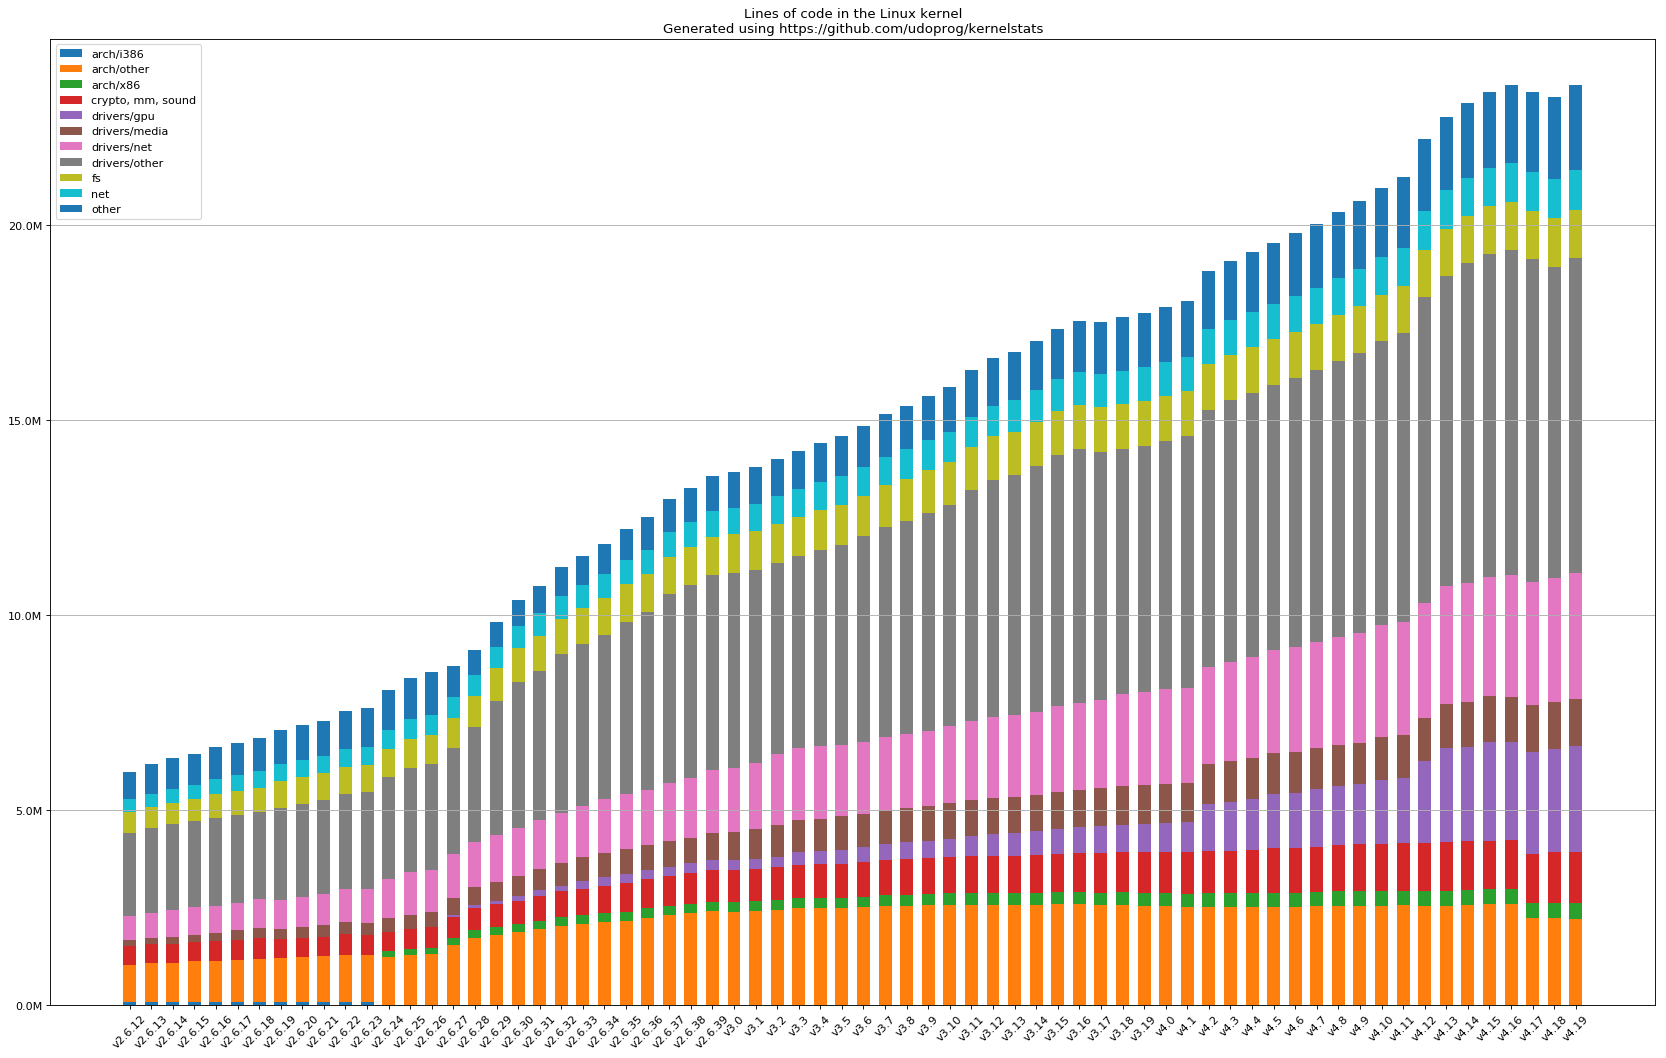
\includegraphics[scale=0.3]{figures/linux-loc.png}
    \caption{Lines of code in each version of the Linux kernel \cite{kernel-stats}}
    \label{linux-growth}
\end{figure}

The developers had only intended to use BKL to ease the initial transition to multicore. They then began making an effort to transition towards finer-grained locking, aiming to protect each data structure with an individual lock and eventually remove the BKL \cite{locking-smp-kernels}. However, changes to the locking code had to be implemented very cautiously, to avoid introducing difficult-to-detect deadlocks. The problem was exacerbated by the sheer scale of the Linux kernel project. As an illustration, the graph shown in figure \ref{linux-growth} shows the growth of the source code with each release, and as of January 2020, the kernel comprised 27.8 million lines of code \cite{linux-loc}. It was a long and difficult task to map the semantics of such a large codebase and refactor it to use finer-grained locking, and every additional fine-grained lock increased the complexity. It wasn't until version 2.6.39 of the kernel was released in May 2011 that the BKL was finally removed, some 15 years after it was first introduced. If the developers had the opportunity to redesign Linux with multicore in mind, this time would have been greatly reduced. However, once an operating system is established, redesign is not a feasible option. The cost of redeveloping Linux was estimated in 2011 at \$3 billion USD, and again in 2018 at \$14.7 billion USD \cite{cost-to-redev}.  

One of the main benefits of Linux, particularly for education, is the open-source nature of the project. However, the large and complex nature of the project makes it almost impossible for a novice programmer to understand. Furthermore, Linux is mostly written in C, which has no support for object-oriented concepts. However, developers do use structs within the Linux source code to mimic a semi-object oriented nature. Since a C struct can combine data items of different kinds, the struct can hold multiple data values, representing the attributes of an object, and multiple pointers to functions, representing the methods of an object. Inheritance and polymorphism can also be achieved, offering great flexibility, but demanding a good grasp of low-level programming concepts such as pointers. Furthermore, the documentation is not yet cohesive, with the community still working to integrate separate documents into a coherent whole \cite{linux-docs}. In essence, the semi-object oriented nature of Linux is very powerful, but is not specifically designed to be easily understood, particularly by novice programmers.

\subsubsection{Barrelfish}
Maybe?

\subsection{InfOS} \label{infos-introduction}
InfOS \cite{infos} is a research operating system, written entirely from scratch in C++ following an object-oriented design. It is based on the x86 architecture, and was designed and developed by Tom Spink for the UG3 Operating Systems course \cite{ug3os}, although it is technically a general purpose operating system. InfOS was designed precisely because modern operating system kernels like the Linux kernel are extremely complex and difficult to understand. It is a valuable teaching tool that forms the foundations of the Operating Systems coursework, providing interfaces for core operating system operations, allowing students to rewrite different subsystems like the memory allocator or the scheduler, developing their understanding of operating system internals. InfOS currently only supports single core processing, but being relatively lightweight in comparison to the operating systems discussed above, InfOS presents a unique opportunity to redesign an operating system specifically with multicore processing in mind. 

\subsection{Key Contributions} \label{key-contributions}
The object-oriented design of InfOS will extend naturally to support multicore processing in a well-structured manner, and adding this support will develop InfOS further as a teaching and research tool. If successful, this project will provide two key contributions:

\begin{itemize}
    \item A well-designed, object-oriented multicore operating system that can be easily understood by students. As discussed, multicore processing is a very pervasive field, and thoroughly understanding parallel architectures is vital for computer science students, especially those interested in systems development.
    \item A platform on which to build further research. The multicore implementation will extend the way InfOS provides interfaces for components of the operating system, allowing experimentation with different algorithms to balance the system's workload between cores and performance optimisation. See section \ref{future-work} for further discussion.
\end{itemize}

\chapter{Implementation} \label{implementation}

\section{Existing system} \label{existing-system}
As described in section \ref{motivation}, InfOS has a clear advantage over other operating systems because it was designed to be straightforward to understand. With this being said, InfOS is still a general purpose operating system, and the whole repository comprises around 20,000 lines of code. Before implementation could begin, the major conceptual challenge was to understand the existing system. There is a brief specification document (ref ??? learn) written by the designer, which is aimed at students of the UG3 operating systems course and explains InfOS’s high-level structure and implementation, but it is by no means extensive technical documentation. Most of my understanding of InfOS therefore came from navigating the existing codebase and reading the Intel architecture manuals \cite{intel-full-manual}. This consumed a significant portion of development time throughout the entire project. Another conceptual challenge was that the C++ standard library was unavailable, meaning that the entire implementation had to be written in the C++ core language \cite{cpp-core}. This is because the standard library implementation makes use of syscalls, and therefore must be ported to each individual operating system. Naturally, no such port exists for InfOS, so functionality including strings, lists, maps, input/output, random number generation, atomics support and time utilities were not supported. While InfOS does already implement its own versions of string, list and map, any other standard C++ functionality needed during the implementation had to be written from scratch. This became particularly relevant when atomic operations were needed (see section \ref{scheduling-threads} for further details).
 
The Advanced Programmable Interrupt Controller (APIC) \cite{intel-sys-prog-guide} is the Intel standard for processors, and InfOS is an APIC-based system. The standard defines two main controllers, a local APIC (LAPIC) and an external input/output APIC (I/O APIC). The I/O APIC is responsible for receiving external I/O interrupts, such as keyboard strokes, and relaying them to the LAPIC. Each LAPIC has an LAPICTimer, and the LAPIC is responsible for receiving internal I/O interrupts such as LAPICTimer interrupts, alongside the I/O APIC generated interrupts. APIC supports multiprocessor systems by representing each processor as a core and an LAPIC, with each LAPIC handling core-specific interrupts. With this representation, the system has one I/O APIC, and as many LAPICs and LAPICTimers as there are cores. The cores may communicate by sending Inter-processor Interrupts (IPIs) from their LAPIC to another processor’s LAPIC \cite{intel-sys-prog-guide}. InfOS has an object-oriented design, with each of the major components of the operating system represented as a subclassed device object. For example, the scheduler, I/O APIC and LAPIC are all represented as devices. When InfOS boots, the platform is probed, and any detected devices are created during and registered with the device manager. Every device is assigned a unique name by the device manager, who is then responsible for providing an interface that allows any class of device to be accessed by other parts of the system. The most natural design extension was to represent the cores as objects, with each core having a separate LAPIC and LAPICTimer object. With this design in mind, I broke the implementation down into four main milestones:

\begin{description}
\item [Detecting cores.] QEMU \cite{qemu} is a virtualisation environment that can be used to boot real operating systems in a virtual machine, and was used throughout development to emulate running InfOS. This allowed me to easily configure the processor architecture to emulate, specifically the number of cores. The first milestone, then, was to supply InfOS with multiple cores and detect those cores during boot up.

\item [Initialising cores.] As previously mentioned, the x86 ISA defines a MP initialisation protocol, which defines two classes of processors, the bootstrap processor (BSP) and application processors (APs). The BSP runs the main operating system boot code, and is responsible for the previous detection of other cores. When the AP cores boot, they are initially in a waiting state, so the BSP is also responsible for sending IPIs to those APs to give them something to do. The role of initialising the cores, then, is to give them a stack and a memory address to start execution at. For the purpose of this milestone, the code can be general code, such as “Hello world from core x!”.

\item[Calibrating timers.] InfOS already supports preemptive scheduling. This is achieved by LAPICTimer interrupts every millisecond triggering a scheduling event. Therefore, each core’s timer had to be calibrated and initialised to send periodic interrupts. The calibration code determines the frequency of the timer by measuring it against the programmable interrupt timer (PIT), meaning that the calibration code must be executed on the core itself to determine the correct frequency. Therefore, it made sense to do the timer calibration once each core was awake and running general code, and this was the third milestone.  

\item[Scheduling threads.] On every timer interrupt, a scheduler event occurs, so the next logical step once each core was taking timer interrupts was to configure the scheduler to recognise multiple cores and dispatch tasks between them. Once this was implemented, all threads running in the operating system would need to be shared between the cores. There was a lot of design decisions to be made here, such as how to share the threads between the cores and whether a centralised scheduling manager should be used to coordinate.
\end{description}

\section{Detecting cores} \label{detecting-cores}
As already mentioned, QEMU provides a simple way to modify the number of cores available to InfOS via the \verb|-smp| argument. For instance, InfOS can run on a dual-core processor by adding the command line argument \verb|-smp 2| to the run script. Once provided with multiple cores, however, InfOS still has to detect them. The Advanced Configuration and Power Interface (ACPI, not to be confused with the previously mentioned Advanced Programmable Interrupt Controller, APIC) provides an open standard that operating systems can use to discover and configure hardware components. To begin using ACPI, the operating system must locate the Root System Description Pointer (RSDP), which contains a pointer to the Root System Description Table (RSDT), which contains pointers to yet more tables describing the hardware available on the system. InfOS already had an implementation to locate the RSDP, enable ACPI and parse the tables, so I extended this existing code to collect information about the available cores. 

One of the tables pointed to by the RSDT is the Multiple APIC Description Table (MADT), which describes all of the interrupt controllers in the system. Each entry in the MADT has an entry type, and entry type 0 is used to represent LAPICs, as shown in figure \ref{madtentry0}. 

\begin{figure}[h]
    \centering
    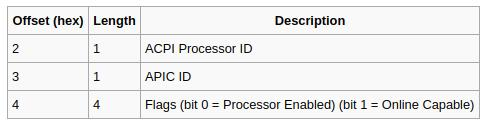
\includegraphics[scale=0.7]{madtentry0.jpg}
    \caption{MADT Entry Type 0 \cite{osdev-madt}}
    \label{madtentry0}
\end{figure}

Since each core has its own LAPIC, each core's LAPIC will be represented by an individual MADT entry of type 0. Each entry contains the processor's ID, the LAPIC's ID and a set of flags. The flags are represented as 32 bits (see figure \ref{entry0flags}) and contain extremely important information: whether or not the processor can be enabled. If bit zero is set, the processor is enabled. If bit zero is clear, but bit one is set, then the system supports enabling the processor during OS runtime. If neither bit is set, then there is some error with the processor, meaning that it cannot be enabled and the OS should not try.

\begin{figure}[h]
    \centering
    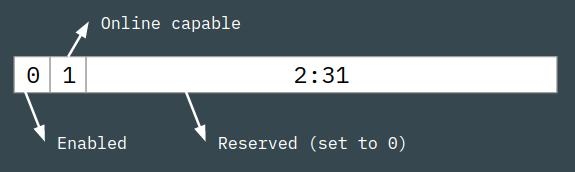
\includegraphics[scale=0.6]{figures/entry0flags.jpg}
    \caption{Entry type 0 flags structure}
    \label{entry0flags}
\end{figure}

It is useful to know which core is the BSP (for timing purposes, discussed further in section \ref{calibrating-timers}), so this information needs to be recorded at some point during core detection or core initialisation. The simplest way is to record the ID of the BSP, which can be done by reading the ID register of the BSP's LAPIC. Every core's LAPIC registers are memory-mapped to the same base address, and this base address is specified in the MADT. This mapping means that each core is only able to directly access its own LAPIC registers, so reading the BSP's LAPIC ID register must be done by code executing on the BSP. At this stage of boot, only the BSP is executing code while the APs sit idle, so the core running the code parsing the ACPI tables is guaranteed to be the BSP. For this reason, it makes sense to collect the BSP ID at this point by reading the LAPIC ID register, and store it for later.

As already discussed, the object-oriented design of InfOS extends well to supporting multiple cores. I decided to represent each core as a new subclass of device, creating and registering a new core object with the device manager whenever an entry type 0 was encountered in the MADT table. Within the core object, I stored the LAPIC ID, needed later for sending inter-processor interrupts between cores, and the core state. The core state is represented by an enum with four values, \verb|BOOTSTRAP|, \verb|ONLINE|, \verb|OFFLINE|, and \verb|ERROR|, and is used during the core initialisation process to decide whether or not to send the wake sequence of IPIs to the core. If bit zero and bit one are both clear, the core state is set to \verb|ERROR| so that the core is not enabled later. Otherwise, the core's state is set to \verb|OFFLINE|, with this being changed to \verb|ONLINE| once the initialisation sequence is complete. The only exception is the case when the core's ID matches the BSP's ID, in which case the state is set to \verb|BOOTSTRAP|. Note that state \verb|BOOTSTRAP| implies the state \verb|ONLINE|, since if we have reached this stage in the boot process, the BSP is already executing code.

\section{Initialising cores} \label{initialising-cores}
Once the APs have been detected, they need to be triggered to begin execution. The BSP can generate interprocessor interrupts (IPIs) by writing specific values to one of its LAPIC registers, the interrupt command register (ICR). As already mentioned, each core is able to directly access its own LAPIC registers by writing to the LAPIC base address plus some offset. The ICR comprises two 32-bit registers, one at offset \verb|0x300| and the other at offset \verb|0x310|. The Intel MP protocol defines a sequence of IPIs, called an INIT-SIPI-SIPI sequence, that wakes a processor from the waiting state. To send an Initialisation (INIT) IPI, the BSP first writes the target LAPIC ID into bits 24-27 of offset \verb|0x310|, then writes the value \verb|0x00004500| to offset \verb|0x300|, which generates the interrupt. To send a Startup IPI (SIPI), the target LAPIC ID is written as before, and then the value \verb|0x00004600| is or-ed with the page number at which the AP should begin executing, before being written to offset \verb|0x300|. The initialisation sequence then proceeds as follows: the BSP sends an INIT IPI to the AP, waits 10 milliseconds, sends a SIPI and then waits a further 1 millisecond. The BSP then polls for a ready flag from the AP indicating that it is online. If the ready flag is not set, the BSP repeats the SIPI and waits a further 1 second. If the ready flag is still not set after the second, the core state is set to \verb|ERROR| and the BSP stops trying to wake that core.

The page address sent with the SIPI locates initialisation assembly code, commonly referred to as trampoline code. The BSP allocates page zero as the trampoline page and copies the assembly code onto that page, before including the address of that page with the SIPI. For compatibility reasons, all x86 processors begin execution in 16-bit real mode, a simplistic mode used by early operating systems with only 1MB of addressable memory, no memory protection and no virtual memory. The main operating mode of Intel processors today is 64-bit protected mode, so the trampoline code must enable this on the AP. In protected mode, memory access is controlled through the Global Descriptor Table (GDT), which stores information about various memory areas, their base address, size and access privileges. Therefore, before entering protected mode, the AP must first prepare a temporary GDT to access. Once the GDT is ready, protected mode is enabled by setting the \verb|PE| control flag in the \verb|CR0| register. In a similar fashion, interrupt handling is controlled through the Interrupt Descriptor Table (IDT), so the AP must also load this table using the \verb|lidt| instruction.

The AP is now executing in protected mode, but it is not yet finished initialising. InfOS uses paging, so this must also be enabled on the AP. However, before paging is enabled, the page directory address needs to be loaded into the AP's \verb|CR3| register so that the AP can locate the page table. The trampoline code reserves some storage space for this value in the data segment, and then the BSP inserts this value when copying the trampoline code to page zero. The AP then loads this value from the data segment into its \verb|CR3| register, and paging is enabled by setting the \verb|PG| flag in the \verb|CR0| register. Additionally, each AP needs its own stack, so the BSP allocates the AP one page of memory and again inserts a pointer to this page in the data segment. The AP can then load this value into its \verb|RSP| register, at which point, the AP is finished using the trampoline code. There is one final reserved storage location for the previously mentioned ready flag, which the AP sets and the BSP polls for. Finally, the AP jumps to a function \verb|x86_core_start|, which prints \verb|"Hello world from core x!"| to the terminal and then pauses indefinitely. A six core system (with one BSP and five APs) would give the console output shown in figure \ref{hello-world}.

\begin{figure}[h]
    \centering
    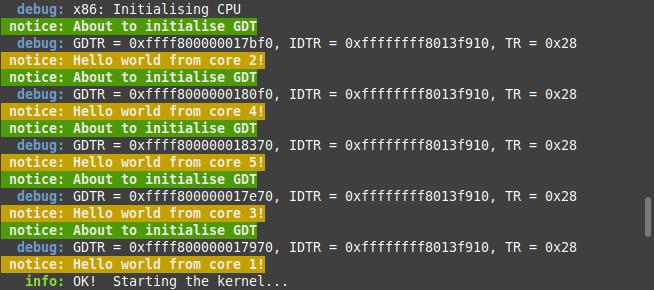
\includegraphics[scale=0.6]{figures/hello-world.jpg}
    \caption{Console output when initialising a six core system}
    \label{hello-world}
\end{figure}


The sequence described above needs to be done for each core individually, and this can either be done in serial or in parallel. Serial initialisation has one trampoline page that each AP uses in turn, with the BSP waiting for one AP to complete initialisation before broadcasting the INIT-SIPI-SIPI sequence to the next AP. This introduces a bottleneck that could be reduced by giving each AP a separate trampoline page and broadcasting the INIT-SIPI-SIPI sequence across the bus to start all present cores. However, this will wake any present core, irrespective of the value of the core's ready flags found in the MADT, which could potentially wake a core that had previously been deliberately disabled due to an error. For this reason, broadcasting is generally avoided during AP initialisation, so I decided to do the initialisation serially. The BSP retrieves the list of available cores from the device manager and only sends IPIs to \verb|OFFLINE| cores. The BSP has to then wait for each core to set the ready flag before either resending the SIPI or moving on and updating the core's state. The initialisation code is relatively small because InfOS is so lightweight, meaning that this serial initialisation process has a negligible impact on overall system performance.

\section{Calibrating timers} \label{calibrating-timers}
As well as the cores, each AP's LAPIC and LAPICTimer also need to be registered with the device manager, and additionally the LAPICTimer needs to be calibrated to determine the frequency.
Once the APs are executing code, the next step is to calibrate 

\section{Scheduling threads} \label{scheduling-threads}


\chapter{Evaluation}

As discussed in section \ref{scalability-challenges}, in order to fully exploit the processing power of multiple cores, software needs to be highly adapted to a parallel execution environment. An embarrassingly parallel problem is one where very little effort is needed to divide the original task into a set of almost independent parallel tasks, and such problems are both pervasive in computing and well-suited to exploiting parallel architectures. 

\begin{figure}[h]
    \centering
    
\includegraphics[scale=0.15]{mandelbrot-bw.jpg}
    \caption{Black and white rendering of the Mandelbrot set \cite{mandelbrot-bw}}
    \label{mandelbrot-bw}
\end{figure}

\section{The Mandelbrot Set}
The Mandelbrot set is the set of complex numbers $c$ for which the recurrence relation $f_{c}(z) = z^2 +c$ with $z_{0}=0$ does not diverge. Thus, a complex number $c$ is a member of the Mandelbrot set if, when applying $f_{c}$ repeatedly, the absolute value of $z_{n}$ remains bounded for all $n>0$. The set can be represented visually in a two-dimensional plane by taking each $(x,y)$ point in the plot as the real and imaginary parts of a complex number $c$, such that $c=x+iy$, and iteratively computing values for the recurrence relation $f_{c}$. An arbitrary escape value is chosen, and each iteration checks whether the result has exceeded this critical value. If the escape value has been exceeded, the computation has diverged and that pixel is not a member of the Mandelbrot set, so computation for that particular pixel can terminate. Otherwise, computation continues until a number of maximum iterations, at which point it is inferred that the pixel will probably not diverge and is a member of the Mandelbrot set. A simple black and white rendering like figure \ref{mandelbrot-bw} can then colour a pixel black if it does not diverge, or white if it does diverge. A coloured rendering can provide additional detail by recording how many iterations it takes each pixel to diverge and colouring each pixel correspondingly. This gives a representation of how fast each pixel diverges, as shown in figure \ref{mandelbrot-vis}.

\begin{figure}[h]
    \centering
    
\includegraphics[scale=0.6]{mandelbrot.jpg}
    \caption{Coloured rendering of the Mandelbrot set \cite{mandelbrot-set}}
    \label{mandelbrot-vis}
\end{figure}

The algorithm described above is often known as the escape time algorithm \cite{mandelbrot-plotting-algorithms}. It is a perfect example of an embarrassingly parallel problem, because the computation of each pixel is independent from every other pixel in the plane. Separate threads within InfOS could therefore handle the computation of each pixel without the need for any communication, making this an ideal benchmark to measure how introducing additional cores affects performance.

\section{The Mandelbrot Benchmark} \label{mb-benchmark}
\subsection{Experimental Environment} 
I wrote a benchmark program in the userspace that computes and displays the Mandelbrot set in the InfOS shell. The program takes the number of threads as a parameter and distributes the computational work evenly between them, which allowed me to vary both the number of cores and the number of threads for each execution. One simple way to divide the work between threads this would be to divide the plane into equal sections and have each thread compute all the pixels within a section independently, but it is important to note that this would not be an equal division of work because pixels require differing amounts of work to compute. Some pixels may diverge very quickly, after a handful of iterations, whereas others may take longer to diverge or not diverge at all, running for thousands of iterations until the maximum iterations limit is reached. To distribute the work more evenly, the program instead uses a global \verb|next_pixel| variable which ranges from \verb|0| to \verb|80x25|, or \verb|2000|. The requested number of threads are then created, and when a thread has no work to do, it atomically reads the value of \verb|next_pixel| and increments it using a \verb|fetch_and_add| function. The thread is then responsible for computing that pixel, and the $(x,y)$ values are retrieved using \verb|x=next_pixel%80| and \verb|y=next_pixel/25|. The colour for each pixel is decided based on the number of iterations, and a \verb|*| character of that colour is printed directly to the shell at the correct $(x,y)$ position. This results in an output like figure \ref{terminal-output}.

\begin{figure}[h]
    \centering
    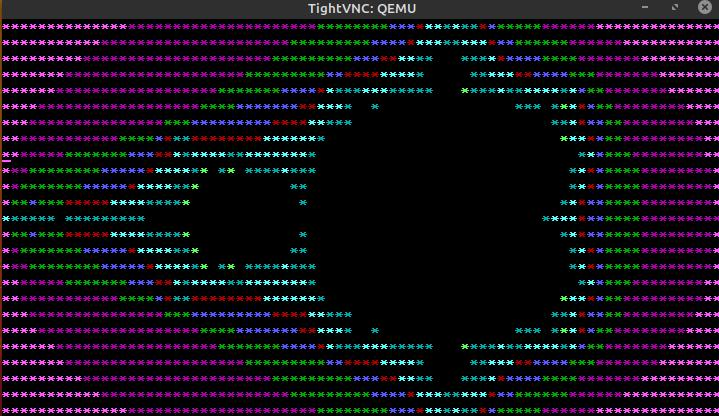
\includegraphics[scale=0.6]{figures/terminal-output.jpg}
    \caption{Rendering of the Mandelbrot set in the InfOS shell}
    \label{terminal-output}
\end{figure}

It is important that the function \verb|fetch_and_add| is atomic to ensure that no race conditions arise when two threads attempt to access \verb|next_pixel| at the same time. As already mentioned, InfOS does not have access to the standard C++ library with atomics support, so this \verb|fetch_and_add| function was written in userspace using x86 assembly instructions, specifically \verb|xaddl|, by Tom Spink. The use of this \verb|next_pixel| variable ensures that all threads are kept busy until the entire plane has been computed, maximising throughput. \\

One other important point to note is that the Mandelbrot set is traditionally computed using floating point arithmetic. While InfOS does have a floating point unit, it does not routinely save and restore the floating point registers during a context switch in order to reduce switching overhead. This means that with a multithreaded execution of the benchmark, any floating point computation would be overwritten and interfered with by other threads unless the floating point state was saved. We did spend some time trying to save floating point state on a context switch with the \verb|xsave| instruction, but this turned out to be more complex than expected and we weren't able to implement this past the unicore case within the time available. Because the focus of this project is parallel computation rather than floating point arithmetic, we instead decided to implement the Mandelbrot algorithm using fixed-point arithmetic and left the floating point context switching as future work. A fixed-point number representation simply stores all values multiplied by some normalisation factor, uses integer operations for calculations, and then normalises the result when required. By choosing the multiplier to be a power of 2, I was able to compute the Mandelbrot set using only integer operations, and then use bit shifting operations to quickly perform multiplication and division when necessary. \\

As already discussed, the program supported varying the number of threads alongside the number of cores, since for $x$ cores to be utilised effectively, there must be at least $x$ independent threads ready for execution. This allowed me to experiment with the following three scenarios:

\begin{enumerate}
    \item Single core, single-threaded 
    \item Single core, multithreaded 
    \item Multicore, multithreaded
\end{enumerate}

The single core, single-threaded case provided a baseline for execution time to compare against. It was important to separate the two multithreaded cases because even in the single core case, multithreading alone can improve performance. For example, CPU throughput can be increased by replacing a blocked thread with one that is ready to execute, until the blocked thread is ready to resume execution. In order to determine if any performance difference was produced by making the Mandelbrot program multithreaded or by introducing additional cores, it was important to isolate the changes between experiments cases. The combinations of threads and cores used can be seen in figure \ref{cores-threads}, with horizontal lines separating the three cases. For each configuration, I timed the real execution time using a timing program written by Tom Spink. This timing program was verified using an external stopwatch to ensure accuracy. Each parameter configuration was executed three times, and then the execution times were averaged, to give the results shown in \ref{timing-infos-mb}. \\

\subsection{Results} \label{mb-benchmark-results}
todo: interpret these bad boys

\begin{table}[h]
    \centering
    \begin{tabular}{cl}
         Cores & Threads \\
         \toprule
         1 & 1 \\
         \midrule
         1 & 2, 4, 8, 16, 32 \\
         \midrule
         2 & 2, 4, 8, 16, 32 \\
         3 & 2, 4, 8, 16, 32 \\
         4 & 2, 4, 8, 16, 32 \\
    \end{tabular}
    \caption{Configuration of core and thread counts used for experiments}
    \label{cores-threads}
\end{table}


\begin{table}[h]\centering
\caption{Mandelbrot timing!}\label{timing-infos-mb}
\scriptsize
\begin{tabular}{ccc}\toprule
Cores &Threads &Average (s) \\
\midrule
1 &1 &9.143 \\
\midrule
1 &2 &9.150 \\
1 &4 &9.400 \\
1 &8 &9.387 \\
1 &16 &9.243 \\
1 &32 &9.430 \\
\midrule
2 &2 &4.753 \\
2 &4 &4.930 \\
2 &8 &4.950 \\
2 &16 &4.887 \\
2 &32 &4.873 \\
\midrule
3 &2 &\textbf{4.900} \\
3 &4 &3.453 \\
3 &8 &3.447 \\
3 &16 &3.377 \\
3 &32 &3.390 \\
\midrule
4 &2 &\textbf{4.910} \\
4 &4 &2.647 \\
4 &8 &2.670 \\
4 &16 &2.677 \\
4 &32 &2.687 \\
\bottomrule
\end{tabular}
\end{table}

\section{The Modified Mandelbrot Benchmark} \label{mb-mod-benchmark}
\subsection{Experimental Environment} 
As expected, the more cores available to InfOS, the better the performance. However, I wanted to compare this performance scaling to a highly-developed and well-established operating system in order to visualise how efficiently InfOS uses the additional available resources. To do this, I ported the Mandelbrot benchmark into a Linux version. Since the pixels may be computed out of order, the original Mandelbrot benchmark displays the output to the terminal correctly by allowing each thread to specify exactly which $(x,y)$ point to print which colour to. There is no way to do this in standard C++ without writing additional complex functionality, so the benchmark was modified to save the pixel value to a global two-dimensional array, rather than printing the value to the screen. I controlled the number of threads by creating pthreads, and I controlled the number of cores by affining those threads to a CPU set: so in the single core case, all threads were affined to a singleton CPU set, in the dual core case, all threads were affined to a CPU set containing two cores, and so on. \\

I then reran the same core and thread configurations as in table \ref{cores-threads} on InfOS, but using the modified Mandelbrot benchmark. I also ran this modified Mandelbrot benchmark on Linux, again with the same core configurations as in table \ref{cores-threads}. I timed the Linux execution using the \verb|time| command, and again, verified this with an external stopwatch to ensure accuracy. In order to ensure fairness, the frequency of InfOS was changed from 100Hz to 250Hz, to match Linux's value. This ensured that both operating systems were taking the same number of timer interrupts per second, and therefore had the same interrupt handling overhead. I also manually set the Linux scheduler to be FIFO and gave the threads maximum priority, to ensure they had the best possible chance of executing quickly. This gave the results shown in tables \ref{timing-infos-mb-mod} and \ref{timing-linux-mb-mod}.

\subsection{Results}
todo: interpret
\begin{table}[h]
\label{timing-infos-mb-mod}
\parbox{.45\linewidth}{
\centering
\scriptsize
\begin{tabular}{ccc}
\toprule
Cores &Threads &Average (s) \\
\midrule
1 &1 &9.210 \\
\midrule
1 &2 &9.200 \\
1 &4 &9.378 \\
1 &8 &9.367 \\
1 &16 &9.135 \\
1 &32 &9.273 \\
\midrule
2 &2 &4.539 \\
2 &4 &4.736 \\
2 &8 &4.763 \\
2 &16 &4.587 \\
2 &32 &4.644 \\
\midrule
3 &2 &\textbf{4.678} \\
3 &4 &3.228 \\
3 &8 &3.260 \\
3 &16 &3.184 \\
3 &32 &3.266 \\
\midrule
4 &2 &\textbf{4.676} \\
4 &4 &2.429 \\
4 &8 &2.457 \\
4 &16 &2.473 \\
4 &32 &2.451 \\
\bottomrule
\end{tabular}

\caption{Infos mandelbrot modified description}
}
\hfill
\parbox{.45\linewidth}{
\centering
\label{timing-linux-mb-mod}
\scriptsize
\begin{tabular}{ccc}
\toprule
Cores &Threads &Average (s) \\
\midrule
1 &1 &8.937 \\
\midrule
1 &2 &8.864 \\
1 &4 &8.708 \\
1 &8 &8.857 \\
1 &16 &8.866 \\
1 &32 &8.873 \\
\midrule
2 &2 &4.584 \\
2 &4 &4.572 \\
2 &8 &4.542 \\
2 &16 &4.449 \\
2 &32 &4.466 \\
\midrule
3 &2 &\textbf{4.578} \\
3 &4 &3.079 \\
3 &8 &3.158 \\
3 &16 &3.162 \\
3 &32 &3.185 \\
\midrule
4 &2 &\textbf{4.563} \\
4 &4 &2.432 \\
4 &8 &2.382 \\
4 &16 &2.359 \\
4 &32 &2.426 \\
\bottomrule
\end{tabular}
\caption{linux mandelbrot modified description}
}
\end{table}

todo: make this less shit
\pgfplotstabletypeset{infos-timing.txt}
\begin{tikzpicture}
\begin{axis}[xlabel=Number of Cores, ylabel=Time in seconds]
\addplot table [y=Average, x=Cores]{infos-timing.txt};
\end{axis}
\end{tikzpicture}

\section{The Cache Benchmark} \label{cache-benchmark}
\subsection{Experimental Environment}
As well as investigating how performance scaled with added resources, I wanted to evaluate the impact of different workload management on performance. Recall that section \ref{scheduling-challenges} discussed that after a thread has been running on a specific core, that core's private cache will hold relevant data to that thread. An increased number of cache hits leads to better performance, so the thread is said to have an affinity for that core. Section \ref{scheduling-challenges} also discussed the issue of keeping the workload balanced between cores, such that no one core is sitting idle while other cores are overwhelmed. With a system-wide ready queue, the load would have been naturally balanced, and with a per-core ready queue, the affinity problem would have been provided for free, but as discussed in section \ref{scheduling-threads}, I chose to take a hybrid approach, having a global scheduling manager dispatch threads to particular cores. When a thread blocks and then becomes ready again, it goes back to the global scheduling manager, who may choose to dispatch it to a different core to resume execution. This hybrid approach allowed more flexibility for experimenting with different approaches and evaluating the impact of load balancing and processor affinity on performance. \\

InfOS already supported choosing the individual scheduling policy (e.g. round-robin, first-in-first-out) via the command line, but this only concerned each core's individual scheduler. For example, consider a system with two cores running three threads: T1 and T2 on core 1, and T3 on core 2. If the scheduling policy was set to round-robin at boot time, the cores would schedule their own threads according to that policy, so core 1 would execute T1, T2, T1, T2 and so on, and core 2 would execute T3 only. If another thread, T4, were to be created, the global scheduling manager may now choose to dispatch T4 to either core 1 or core 2. Dispatching T4 to core 2 may seem like the natural choice to keep the workload balanced, but if T4 had previously been executing on core 1 and had data cached there, the performance benefit gained by using the warm cache may outweigh the imbalanced workload. This benchmark is interested in these decisions made by the global scheduling manager and their impact on performance, but not in the scheduling policies used by the individual cores. For the avoidance of doubt, I will refer to the former as ``core migration policy", and the latter as ``scheduling policy". In order to vary the parameters, I added another command line parameter that selected from one of three core migration policy implementations.

\begin{description}
\item[Random.] Uses the \verb|rdrand| instruction to read a random value and takes this number modulo the number of cores available to the system. Uses this number as an index into the list of cores available.
% \item[Round robin.] Removes a core from the head of the list and appends it to the end of the list. Returns this core as the one to dispatch the task to.
\item[Load balancing.] Asks each core to return the number of threads currently in its private ready queue, and then chooses the core with the smallest workload. This is a naive implementation that involves iterating through the list of cores to find the minimum workload, so in the event of multiple cores with the same number of threads, the one closest to the end of the list is chosen. 
\item[Processor affinity.] Asks each thread if it has an affinity for a particular core. This is done using a variable \verb|bool _proc_affinity| and another variable with a reference to the affined core. The \verb|boolean| variable represents whether or not the core reference has been initialised, so if \verb|_proc_affinity| is set to \verb|true|, the thread is passed to the affined core. If \verb|_proc_affinity| is set to \verb|false|, this is the task's first time executing, and the load balancing algorithm described above is asked to return a core. The thread's affinity variables are then set accordingly.
\end{description}

I then needed to test these different policies on a program involving lots of thread migration and lots of cache accesses. I wrote a benchmark loosely inspired by the Bitcoin proof-of-work algorithm \cite{proof-of-work}, which has a global integer array and a number of threads. Each thread is allocated one section of the array and must repeatedly compute the hash of this section, where the hash is essentially the sum of the elements in the section with some salt value. The salt is incremented on every iteration, which increases the sum until the hash exceeds a certain value. Dividing the array between the threads and requiring repeated calculation of the sum means that each thread is repeatedly accessing the same data, which would benefit from being in the core's private cache. In order to simulate blocking for I/O or waiting for some other event, after each calculation, the thread calls yield to stop executing on the current CPU and return to the global scheduling manager, who can then decide which core to dispatch the task to. This benchmark means that each thread is essentially accessing the same data repeatedly, but potentially migrating between cores and losing access to cached data. \\

\subsection{Results}
todo: actually run these experiments lol

\chapter{Future Work} \label{future-work}
\section{Cache-aware scheduling}
\section{Floating Point}


% use the following and \cite{} as above if you use BibTeX
% otherwise generate bibtem entries
\bibliographystyle{plain}
\bibliography{mybibfile}

\end{document}
